\chapter{Background and Concepts}
In this chapter, we will introduces several main concepts that related to our study.
\section{Agile software development}
\label{agile}
The term "Agile" represents the fast adaptation and response to the changes.\cite{WhatisAg98:online}
The agile software development is new method of software development that implements the ideology of "agile". Agile software development advocate the continuous development of a software teams. The software development under this methodology will have shorter planning/development time before it deliver to the costumers and could better adapted to changes in the environment and requirements.
\par
The agile software development uses iterative way in the development process. Traditional software development process, like waterfall, requires the long and complicated planning process, and a complicated document. Once one phase of the development is done, the teams shouldn't change the output (document and code) of this phase.\cite{cusumano1995beyond} In the contrast, the agile software development aims to satisfy the costumer with early and continuous delivery of the software.\cite{beck2001manifesto}. Early means the shorter time before software delivery. Continuous means the development is not end with the delivery. A delivery means teh end an iteration, together with a demonstration to stakeholders. After delivery, the team continue to next iteration according to the feedbacks it gets from stakeholders. In each iteration, the team not aims to add a major features to the software, rather their goal is to have a working and deliverable release\cite{beck1999embracing}. In the ideology of agile, the best design a the software product come from the the iterative development, rather than the tedious planning.\cite{beck2001manifesto}
\par
The rapid development doesn't means the low software development quality. On the contrast, the quality of software design is highly appreciated in the agile software development. The automatic testing is widely used in Agile. The test cases will be defined and implements from the beginning of the development process. The testing goes through the whole development iteration ensure the software has a high enough quality to be released or demonstrate to costumers at any point of an iteration\cite{Agilesof32:online}.
\par
The agile software development processes includes the collaboration across different groups, ie. bushiness development team, software development team, test team, and costumers. It values more face to face communications\cite{beck2001principles} and feedbacks. The goal for these communications is, firstly to let everyone in the multifunctional agile team understand the whole project, secondly, to receive feedbacks that helps the software in the right development track that align with the requirement of the stakeholders. \cite{beck2001manifesto} 
\par
According to the Manifesto for Agile Software Development, compared with traditional software development, the agile software development value these aspects: \cite{beck2001manifesto}
\begin{itemize}
\item Individuals and interactions over processes and tools.
\item Working software over comprehensive documentation.
\item Customer collaboration over contract negotiation.
\item Responding to change over following a plan.
\end{itemize}
\section{CI/CD}
In the software development, CI/CD refers to continuous integration, continuous delivery and continuous deployment.\cite{Continuo67:online}. As we mentioned in \ref{agile}, the agile software development requires the continuous software quality assurance, and iterative development. Currently, CI/CD is one set of the necessary practices for team to become agile by achieving the requirements above. Figure \ref{fig:cicd} shows the relationship between these 3 practices.
\begin{figure}[h]
    \centering
    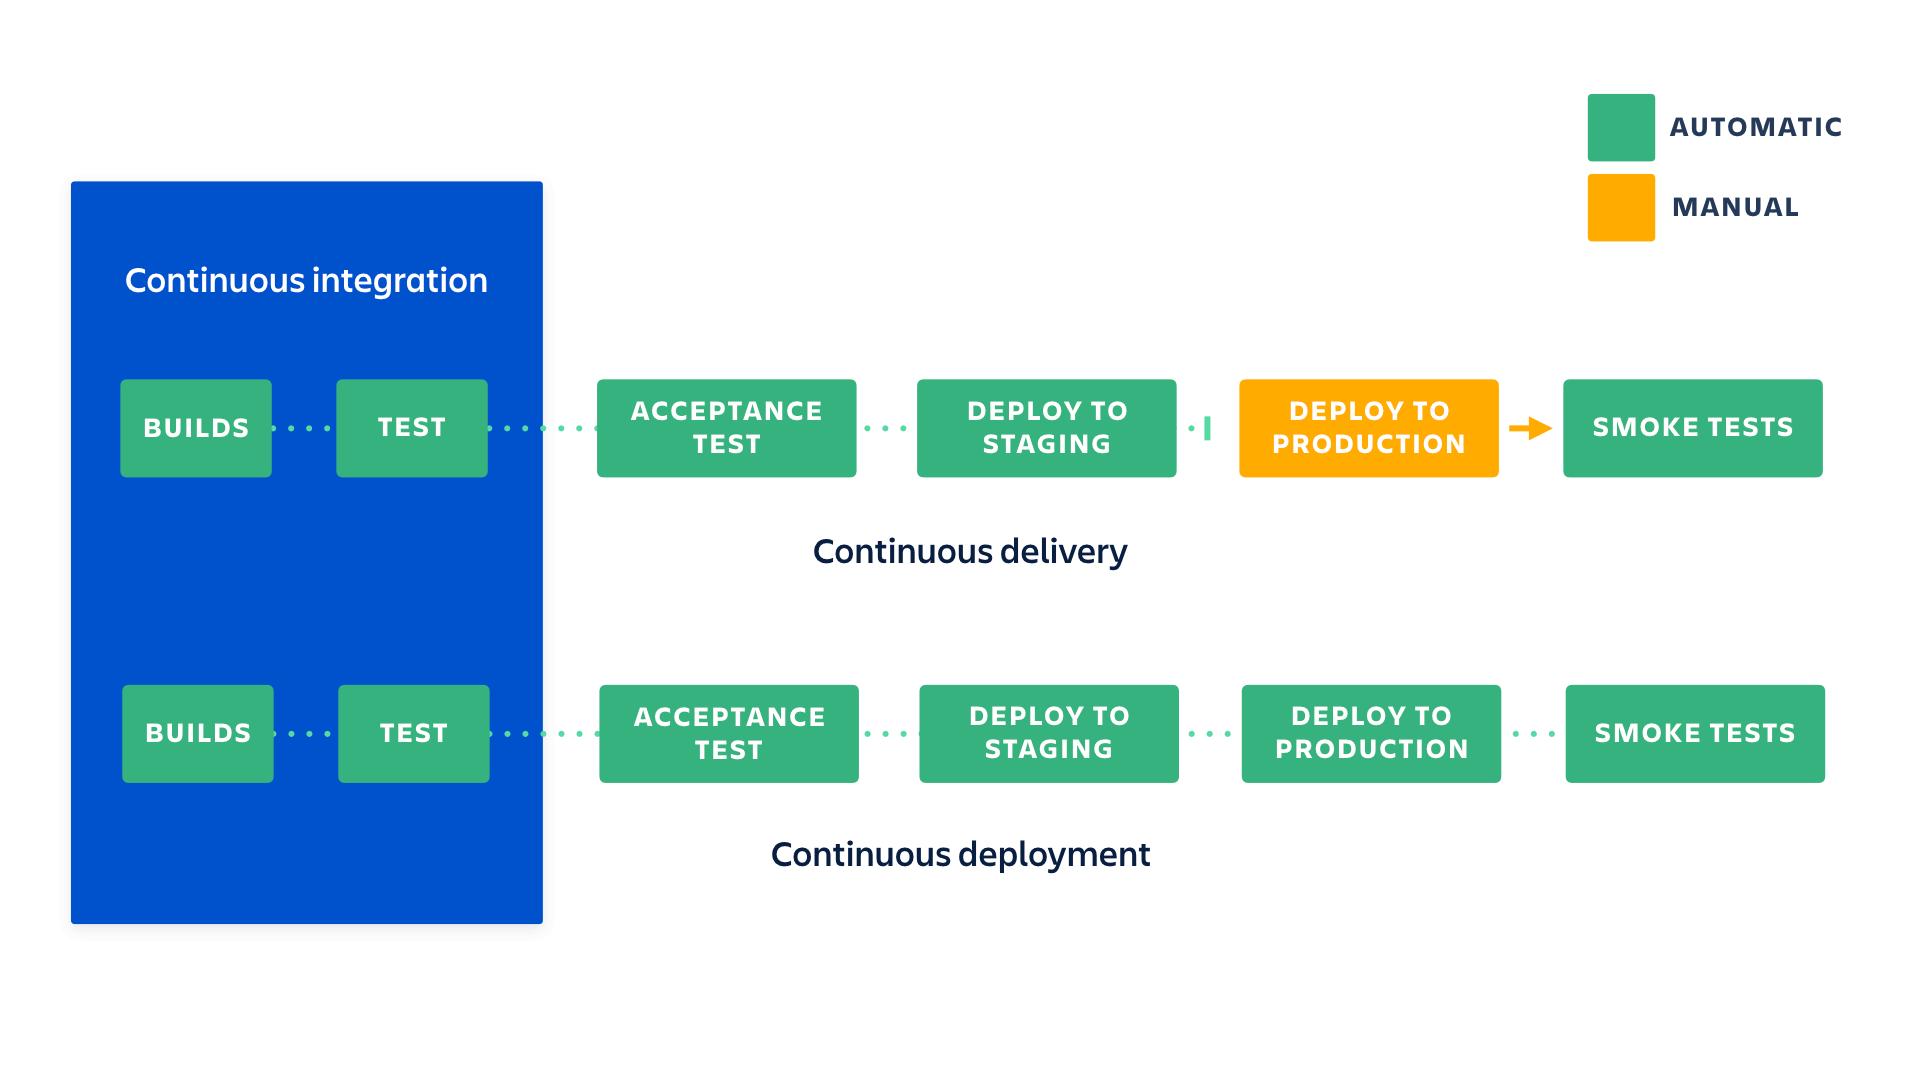
\includegraphics[width=0.95\textwidth]{pics/cicd.png}
    \caption{The relationship between continuous integration, continuous delivery and continuous deployment}
    \label{fig:cicd}
\end{figure}
\subsection{Continuous Integration}
Continuous interaction is the base practice of all practices within CI/CD, and continuous delivery/deployment is based on the continuous interaction.\cite{Continuo67:online}
The continuous integration requires the teams to integrate their work frequently(multiple times per day). "Integrate" means merge the code to the main codebase.\cite{fowler2006continuous}. The continuous interaction rely on 2 practices: \textit{Build Automation} and  \textit{Test Automation}. The definition of these 2 practices are:
\begin{itemize}
    \item \textit{Test Automation:} Test automations means using separate software to execute the software automated, without human intervention. It could helps the team to test fast and test early. \cite{Testauto48:online}
    \item \textit{Build Automation:} Automate the process of creating software build. This means to automate the dependency configuration, source code compiling, packaging and testing. It is viewed as the first step to continuous integration\cite{Buildaut62:online}
\end{itemize}
With the help of these 2 practices, for each developer, the workflow in continuous interaction as follows:\cite{fowler2006continuous} In the development of each feature, the developer first pull the code from the main codebase. During the development, new test cases could also be added to the automated test. After the development is done, the automated testing also runs on the code to maintain the code quality and minimize the number of bugs from the beginning. The build automation compiled the code locally in the development machine. 
\par
Now the developer already have the executable and the high quality (passed the automate test) code in the development machine before submit the change to the code base. This represents the principle of quality and automation in the agile software development. In the next step, the developer commit changes to the repository, which is the main codebase, and the system check the conflict and do the test/build again, to ensure there is not any bugs missed in the test on the development machine.
\section{DevOps}
\section{Tool as Service}
